\documentclass[12pt]{article}
%Fall 2022
% Some basic packages
\usepackage{standalone}[subpreambles=true]
\usepackage[utf8]{inputenc}
\usepackage[T1]{fontenc}
\usepackage{textcomp}
\usepackage[english]{babel}
\usepackage{url}
\usepackage{graphicx}
%\usepackage{quiver}
\usepackage{float}
\usepackage{enumitem}
\usepackage{lmodern}
\usepackage{comment}
\usepackage{hyperref}
\usepackage[usenames,svgnames,dvipsnames]{xcolor}
\usepackage[margin=1in]{geometry}
\usepackage{pdfpages}

\pdfminorversion=7

% Don't indent paragraphs, leave some space between them
\usepackage{parskip}

% Hide page number when page is empty
\usepackage{emptypage}
\usepackage{subcaption}
\usepackage{multicol}
\usepackage[b]{esvect}

% Math stuff
\usepackage{amsmath, amsfonts, mathtools, amsthm, amssymb}
\usepackage{bbm}
\usepackage{stmaryrd}
\allowdisplaybreaks

% Fancy script capitals
\usepackage{mathrsfs}
\usepackage{cancel}
% Bold math
\usepackage{bm}
% Some shortcuts
\newcommand{\rr}{\ensuremath{\mathbb{R}}}
\newcommand{\zz}{\ensuremath{\mathbb{Z}}}
\newcommand{\qq}{\ensuremath{\mathbb{Q}}}
\newcommand{\nn}{\ensuremath{\mathbb{N}}}
\newcommand{\ff}{\ensuremath{\mathbb{F}}}
\newcommand{\cc}{\ensuremath{\mathbb{C}}}
\newcommand{\ee}{\ensuremath{\mathbb{E}}}
\newcommand{\hh}{\ensuremath{\mathbb{H}}}
\renewcommand\O{\ensuremath{\emptyset}}
\newcommand{\norm}[1]{{\left\lVert{#1}\right\rVert}}
\newcommand{\dbracket}[1]{{\left\llbracket{#1}\right\rrbracket}}
\newcommand{\ve}[1]{{\bm{#1}}}
\newcommand\allbold[1]{{\boldmath\textbf{#1}}}
\DeclareMathOperator{\lcm}{lcm}
\DeclareMathOperator{\im}{im}
\DeclareMathOperator{\coim}{coim}
\DeclareMathOperator{\dom}{dom}
\DeclareMathOperator{\tr}{tr}
\DeclareMathOperator{\rank}{rank}
\DeclareMathOperator*{\var}{Var}
\DeclareMathOperator*{\ev}{E}
\DeclareMathOperator{\dg}{deg}
\DeclareMathOperator{\aff}{aff}
\DeclareMathOperator{\conv}{conv}
\DeclareMathOperator{\inte}{int}
\DeclareMathOperator*{\argmin}{argmin}
\DeclareMathOperator*{\argmax}{argmax}
\DeclareMathOperator{\graph}{graph}
\DeclareMathOperator{\sgn}{sgn}
\DeclareMathOperator*{\Rep}{Rep}
\DeclareMathOperator{\Proj}{Proj}
\DeclareMathOperator{\mat}{mat}
\DeclareMathOperator{\diag}{diag}
\DeclareMathOperator{\aut}{Aut}
\DeclareMathOperator{\gal}{Gal}
\DeclareMathOperator{\inn}{Inn}
\DeclareMathOperator{\edm}{End}
\DeclareMathOperator{\Hom}{Hom}
\DeclareMathOperator{\ext}{Ext}
\DeclareMathOperator{\tor}{Tor}
\DeclareMathOperator{\Span}{Span}
\DeclareMathOperator{\Stab}{Stab}
\DeclareMathOperator{\cont}{cont}
\DeclareMathOperator{\Ann}{Ann}
\DeclareMathOperator{\Div}{div}
\DeclareMathOperator{\curl}{curl}
\DeclareMathOperator{\nat}{Nat}
\DeclareMathOperator{\gr}{Gr}
\DeclareMathOperator{\vect}{Vect}
\DeclareMathOperator{\id}{id}
\DeclareMathOperator{\Mod}{Mod}
\DeclareMathOperator{\sign}{sign}
\DeclareMathOperator{\Surf}{Surf}
\DeclareMathOperator{\fcone}{fcone}
\DeclareMathOperator{\Rot}{Rot}
\DeclareMathOperator{\grad}{grad}
\DeclareMathOperator{\atan2}{atan2}
\DeclareMathOperator{\Ric}{Ric}
\let\vec\relax
\DeclareMathOperator{\vec}{vec}
\let\Re\relax
\DeclareMathOperator{\Re}{Re}
\let\Im\relax
\DeclareMathOperator{\Im}{Im}
% Put x \to \infty below \lim
\let\svlim\lim\def\lim{\svlim\limits}

%wide hat
\usepackage{scalerel,stackengine}
\stackMath
\newcommand*\wh[1]{%
\savestack{\tmpbox}{\stretchto{%
  \scaleto{%
    \scalerel*[\widthof{\ensuremath{#1}}]{\kern-.6pt\bigwedge\kern-.6pt}%
    {\rule[-\textheight/2]{1ex}{\textheight}}%WIDTH-LIMITED BIG WEDGE
  }{\textheight}% 
}{0.5ex}}%
\stackon[1pt]{#1}{\tmpbox}%
}
\parskip 1ex

%Make implies and impliedby shorter
\let\implies\Rightarrow
\let\impliedby\Leftarrow
\let\iff\Leftrightarrow
\let\epsilon\varepsilon

% Add \contra symbol to denote contradiction
\usepackage{stmaryrd} % for \lightning
\newcommand\contra{\scalebox{1.5}{$\lightning$}}

% \let\phi\varphi

% Command for short corrections
% Usage: 1+1=\correct{3}{2}

\definecolor{correct}{HTML}{009900}
\newcommand\correct[2]{\ensuremath{\:}{\color{red}{#1}}\ensuremath{\to }{\color{correct}{#2}}\ensuremath{\:}}
\newcommand\green[1]{{\color{correct}{#1}}}

% horizontal rule
\newcommand\hr{
    \noindent\rule[0.5ex]{\linewidth}{0.5pt}
}

% hide parts
\newcommand\hide[1]{}

% si unitx
\usepackage{siunitx}
\sisetup{locale = FR}

%allows pmatrix to stretch
\makeatletter
\renewcommand*\env@matrix[1][\arraystretch]{%
  \edef\arraystretch{#1}%
  \hskip -\arraycolsep
  \let\@ifnextchar\new@ifnextchar
  \array{*\c@MaxMatrixCols c}}
\makeatother

\renewcommand{\arraystretch}{0.8}

\renewcommand{\baselinestretch}{1.5}

\usepackage{graphics}
\usepackage{epstopdf}

\RequirePackage{hyperref}
%%
%% Add support for color in order to color the hyperlinks.
%% 
\hypersetup{
  colorlinks = true,
  urlcolor = blue,
  citecolor = blue
}
%%fakesection Links
\hypersetup{
    colorlinks,
    linkcolor={red!50!black},
    citecolor={green!50!black},
    urlcolor={blue!80!black}
}
%customization of cleveref
\RequirePackage[capitalize,nameinlink]{cleveref}[0.19]

% Per SIAM Style Manual, "section" should be lowercase
\crefname{section}{section}{sections}
\crefname{subsection}{subsection}{subsections}
\Crefname{section}{Section}{Sections}
\Crefname{subsection}{Subsection}{Subsections}

% Per SIAM Style Manual, "Figure" should be spelled out in references
\Crefname{figure}{Figure}{Figures}

% Per SIAM Style Manual, don't say equation in front on an equation.
\crefformat{equation}{\textup{#2(#1)#3}}
\crefrangeformat{equation}{\textup{#3(#1)#4--#5(#2)#6}}
\crefmultiformat{equation}{\textup{#2(#1)#3}}{ and \textup{#2(#1)#3}}
{, \textup{#2(#1)#3}}{, and \textup{#2(#1)#3}}
\crefrangemultiformat{equation}{\textup{#3(#1)#4--#5(#2)#6}}%
{ and \textup{#3(#1)#4--#5(#2)#6}}{, \textup{#3(#1)#4--#5(#2)#6}}{, and \textup{#3(#1)#4--#5(#2)#6}}

% But spell it out at the beginning of a sentence.
\Crefformat{equation}{#2Equation~\textup{(#1)}#3}
\Crefrangeformat{equation}{Equations~\textup{#3(#1)#4--#5(#2)#6}}
\Crefmultiformat{equation}{Equations~\textup{#2(#1)#3}}{ and \textup{#2(#1)#3}}
{, \textup{#2(#1)#3}}{, and \textup{#2(#1)#3}}
\Crefrangemultiformat{equation}{Equations~\textup{#3(#1)#4--#5(#2)#6}}%
{ and \textup{#3(#1)#4--#5(#2)#6}}{, \textup{#3(#1)#4--#5(#2)#6}}{, and \textup{#3(#1)#4--#5(#2)#6}}

% Make number non-italic in any environment.
\crefdefaultlabelformat{#2\textup{#1}#3}

% Environments
\makeatother
% For box around Definition, Theorem, \ldots
%%fakesection Theorems
\usepackage{thmtools}
\usepackage[framemethod=TikZ]{mdframed}

\theoremstyle{definition}
\mdfdefinestyle{mdbluebox}{%
	roundcorner = 10pt,
	linewidth=1pt,
	skipabove=12pt,
	innerbottommargin=9pt,
	skipbelow=2pt,
	nobreak=true,
	linecolor=blue,
	backgroundcolor=TealBlue!5,
}
\declaretheoremstyle[
	headfont=\sffamily\bfseries\color{MidnightBlue},
	mdframed={style=mdbluebox},
	headpunct={\\[3pt]},
	postheadspace={0pt}
]{thmbluebox}

\mdfdefinestyle{mdredbox}{%
	linewidth=0.5pt,
	skipabove=12pt,
	frametitleaboveskip=5pt,
	frametitlebelowskip=0pt,
	skipbelow=2pt,
	frametitlefont=\bfseries,
	innertopmargin=4pt,
	innerbottommargin=8pt,
	nobreak=false,
	linecolor=RawSienna,
	backgroundcolor=Salmon!5,
}
\declaretheoremstyle[
	headfont=\bfseries\color{RawSienna},
	mdframed={style=mdredbox},
	headpunct={\\[3pt]},
	postheadspace={0pt},
]{thmredbox}

\declaretheorem[%
style=thmbluebox,name=Theorem,numberwithin=section]{thm}
\declaretheorem[style=thmbluebox,name=Lemma,sibling=thm]{lem}
\declaretheorem[style=thmbluebox,name=Proposition,sibling=thm]{prop}
\declaretheorem[style=thmbluebox,name=Corollary,sibling=thm]{coro}
\declaretheorem[style=thmredbox,name=Example,sibling=thm]{eg}

\mdfdefinestyle{mdgreenbox}{%
	roundcorner = 10pt,
	linewidth=1pt,
	skipabove=12pt,
	innerbottommargin=9pt,
	skipbelow=2pt,
	nobreak=true,
	linecolor=ForestGreen,
	backgroundcolor=ForestGreen!5,
}

\declaretheoremstyle[
	headfont=\bfseries\sffamily\color{ForestGreen!70!black},
	bodyfont=\normalfont,
	spaceabove=2pt,
	spacebelow=1pt,
	mdframed={style=mdgreenbox},
	headpunct={ --- },
]{thmgreenbox}

\declaretheorem[style=thmgreenbox,name=Definition,sibling=thm]{defn}

\mdfdefinestyle{mdgreenboxsq}{%
	linewidth=1pt,
	skipabove=12pt,
	innerbottommargin=9pt,
	skipbelow=2pt,
	nobreak=true,
	linecolor=ForestGreen,
	backgroundcolor=ForestGreen!5,
}
\declaretheoremstyle[
	headfont=\bfseries\sffamily\color{ForestGreen!70!black},
	bodyfont=\normalfont,
	spaceabove=2pt,
	spacebelow=1pt,
	mdframed={style=mdgreenboxsq},
	headpunct={},
]{thmgreenboxsq}
\declaretheoremstyle[
	headfont=\bfseries\sffamily\color{ForestGreen!70!black},
	bodyfont=\normalfont,
	spaceabove=2pt,
	spacebelow=1pt,
	mdframed={style=mdgreenboxsq},
	headpunct={},
]{thmgreenboxsq*}

\mdfdefinestyle{mdblackbox}{%
	skipabove=8pt,
	linewidth=3pt,
	rightline=false,
	leftline=true,
	topline=false,
	bottomline=false,
	linecolor=black,
	backgroundcolor=RedViolet!5!gray!5,
}
\declaretheoremstyle[
	headfont=\bfseries,
	bodyfont=\normalfont\small,
	spaceabove=0pt,
	spacebelow=0pt,
	mdframed={style=mdblackbox}
]{thmblackbox}

\theoremstyle{plain}
\declaretheorem[name=Question,sibling=thm,style=thmblackbox]{ques}
\declaretheorem[name=Remark,sibling=thm,style=thmgreenboxsq]{remark}
\declaretheorem[name=Remark,sibling=thm,style=thmgreenboxsq*]{remark*}
\newtheorem{ass}[thm]{Assumptions}

\theoremstyle{definition}
\newtheorem*{problem}{Problem}
\newtheorem{claim}[thm]{Claim}
\theoremstyle{remark}
\newtheorem*{case}{Case}
\newtheorem*{notation}{Notation}
\newtheorem*{note}{Note}
\newtheorem*{motivation}{Motivation}
\newtheorem*{intuition}{Intuition}
\newtheorem*{conjecture}{Conjecture}

% Make section starts with 1 for report type
%\renewcommand\thesection{\arabic{section}}

% End example and intermezzo environments with a small diamond (just like proof
% environments end with a small square)
\usepackage{etoolbox}
\AtEndEnvironment{vb}{\null\hfill$\diamond$}%
\AtEndEnvironment{intermezzo}{\null\hfill$\diamond$}%
% \AtEndEnvironment{opmerking}{\null\hfill$\diamond$}%

% Fix some spacing
% http://tex.stackexchange.com/questions/22119/how-can-i-change-the-spacing-before-theorems-with-amsthm
\makeatletter
\def\thm@space@setup{%
  \thm@preskip=\parskip \thm@postskip=0pt
}

% Fix some stuff
% %http://tex.stackexchange.com/questions/76273/multiple-pdfs-with-page-group-included-in-a-single-page-warning
\pdfsuppresswarningpagegroup=1


% My name
\author{Jaden Wang}



\begin{document}
\centerline {\textsf{\textbf{\LARGE{PDE Midterm}}}}
\centerline {Zhuochen (Jaden) Wang, GTID: 903456509}
\vspace{.15in}
\begin{problem}[1]
	We see that $ a = x^2, b = xy, c = y^2$. So $ d = ac - b^2 = x^2 y^2 - (xy)^2 = 0 $, and the matrix $ \begin{pmatrix} a&b\\b&c \end{pmatrix} $ is clearly not identically zero. So the equation is parabolic on $ \rr^2$.

	To change into the standard form, we wish to do an invertible change of coordinate using $ s(x,y)$ and  $ t(x,y)$. Under this transformation, the principal linear part becomes  $ L_0 u = a^* u_{ss} +2b^* u_{st} + c^* u_{tt}$, where $ a^*(x,y) ,b^*(x,y) ,c^*(x,y) $ are the coefficients after applying chain rules. In particular, $ a^*(x,y) = a s_{x}^2 + 2b s_{x}s_y + cs_{y}^2 $. If we wish the $ u_{ss}$ term to vanish, we must set $ a^* =0$. This means that $ s(x,y)$ satisfies the characteristic equation of $ L_0 u$. Let us find all solutions of the characteristic equation. If $ \phi(x,y)$ is such solution, this means that each level set of $ \phi(x,y)$ gives a characteristic curve. Locally, the level set of $ \phi(x,y)$ can be expressed as $y(x) $ (or $ x(y)$ if $ \phi_y=0$) by the implicit function theorem. 
 \begin{align*}
	0=\frac{d\phi}{ dx} &= \phi_x + \frac{d y}{d x} \phi_y  \\
	\frac{d y}{d x} &= - \frac{\phi_x}{ \phi_y} 
\end{align*}
We can then substitute this into $ a^* $. If $ x=0$, then  $ a=0$ which forces $ b=0$. Then for points $ (0,y)$, the equation is already in the standard form. Likewise for $ y=0$. WLOG assume $ x>0$ and $ y>0$. We have
\begin{align*}
	a \left( \frac{d y}{d x}  \right) ^2 + 2b \frac{d y}{d x} + c &= 0 \\
	\frac{d y}{d x} &= \frac{ 2b \pm \sqrt{4b^2-4ac} }{ 2a}  \\
	&= \frac{b\pm \sqrt{b^2-ac} }{ a} \\
	&= \frac{b}{a} \\
	&= \frac{\sqrt{ac} }{ a}  \\
	&= \sqrt{\frac{c}{a}} \\
	&= \frac{y}{ x} 
\end{align*}
	Solving this gives one family of real solutions $ y = C x$ for each level set $ \phi(x,y) = C$. Thus define $ s(x,y) = \frac{y}{x}$ for $ x \neq 0$. Notice that since $ d^* = a^* c^*  - b^* ^2 = -b^* ^2$ is the determinant, which is invariant under a change of basis, $ -b^* ^2 = d = 0$ which forces $ b^* =0$, which also forces $ c^* \neq 0$ since $ A$ is not identically zero and shall remain so under change of basis. Thus we just need to choose an $ t(x,y)$ that is independent from $ s(x,y)$ so the Jacobian is nonsingular. We see that $ t(x,y) = x$ will do, since
	 \begin{align*}
		 \det J = \det  \begin{pmatrix} s_x&s_y\\t_x&t_y \end{pmatrix} = \begin{pmatrix} s_x & \frac{1}{x} \\ 1&0 \end{pmatrix} = -\frac{1}{x} \neq 0 .
	\end{align*}
	It follows that under this change of coordinates, the equation reduces to
	\begin{align*}
		c^* u_{tt} &= 0 \\
		u_{tt} &= 0 
	\end{align*}
	which is in the standard form.
\end{problem}
\begin{problem}[2]
\begin{enumerate}[label=(\alph*)]
\item 
This is Burger's equation so the intuition from homework is that a global solution exists iff $ u_x$ doesn't blow up in finite time. To make this precise, we solve the problem using the method of characteristic first.

The initial curve $ S_0$ is parametrized by $ t_0=0,x_0=s,z_0=u_0(s)$. It is the graph of $ u_0(x)$ over the domain $ \{0\}\times \rr $. From the equation we have $ a=1,b=u,c=-2u$. Since
\begin{align*}
	\det \begin{pmatrix} a&b\\t_0'(s)& x_0'(s) \end{pmatrix} = \det \begin{pmatrix} 1&u\\0&1 \end{pmatrix} = 1 \neq 0 ,
\end{align*}
the projection of $ S_0$ onto $ (t,x)$-plane $ C$ is not characteristic so $ u$ can flow out of the initial curve. Now we can solve the characteristic curves using the characteristic equation:
\begin{align*}
	\begin{cases}
		\frac{dt}{ d \tau}=1, & t(0)=0 \qquad  \implies t = \tau\\
		\frac{d x}{d t}= z, & x(0) = s\\
		\frac{d z}{d t} = -2z,& z(0) = u_0(s) \qquad \implies u(s,t)=z(s,t)=u_0(s) e^{-2t}
	\end{cases}
\end{align*}
For a global solution to exist, intuitively we want $ u$ to flow along characteristic curve for forever. Thus along the characteristic curve, we cannot have  $ u_x$ goes to infinity in finite time, or the flow would terminate. Thus we investigate $ w:= u_x$. Taking partial derivative on both sides of the Burger's equation, we have
 \begin{align*}
	 (u_t+u u_x)_x &= -2u_x \\
	 u_{xt}+u_x^2+u_{x x} &= -2u_x \\
	 w_t + u w_x &= -2 w - w^2 \\
	 \dot{w} &= -2w-w^2 
\end{align*}
Moreover, since $ u_0(s) \in C^{1}(\rr)$, we have $ w(s,0) = \left( u_0 (s) e^{-2 \cdot 0} \right)_x =  u_0'(s)$. Using the method of characteristic again, we see that along the characteristic curve, $ w$ satisfies
\begin{align*}
	\begin{cases}
		\frac{d w}{d t} = -2w-w^2\\
		w(s,0) = u_0'(s)
	\end{cases}
\end{align*}
We compute
\begin{align*}
	- \frac{dw}{ w(w+2)} &= dt \\
	-\frac{1}{2}\left( \frac{1}{w} - \frac{1}{w+2} \right) dw &= dt \\
	\frac{1}{2} \ln |w+2| - \frac{1}{2} \ln |w| &= t+C' \\
	\frac{1}{2} \ln \left| \frac{w+2}{ w} \right| &= t+C' \\
        1+ \frac{2}{w} &= Ce^{2t} \\
	w &= \frac{2}{Ce^{2t}-1} \\
	w(s,0) = \frac{2}{C-1} &= u_0'(s) \\
	C &= \frac{2}{u_0'(s)}+1 \\
	w(s,t) &= \frac{2}{ \left( \frac{2}{u_0'(s)}+1 \right) e^{2t}-1 } 
\end{align*}
We see that for a fixed $ s$ ( \emph{i.e.} on the characteristic curve), $ w(s,t)$ blows up when the denominator approaches 0. This happens when
\begin{align*}
	\left( \frac{2}{u_0'(s)}+1 \right)e^{2t} &= 1 \\
	e^{2t} &= \frac{u_0'(s)}{2+u_0'(s) } \\
	t &= \frac{1}{2} \ln \left( \frac{u_0'(s)}{2+u_0'(s) } \right)
\end{align*}
This is the time of $ w$ blowing up. But if $ \frac{u_0'(s)}{ 2+u_0'(s)} \leq 0 \iff -2 \leq u_0'(s) \leq 0$, or if $t<0 \iff u_0'(s) \geq 0$, then $ t$ would not have a solution in the range $ t\geq 0$ so  $ w$ would not blow up. Therefore, the necessary condition for $ u_0$ is that for all  $ x \in \rr$, $ u_0'(x) \geq -2$. 

We now show that this is also the sufficient condition. Suppose the condition is true. Notice that since $ u_0(x)$ has bounded $ C^{1}$-norm, $ u(x,0)$ is Lipschitz continuous in $ x$. Along each characteristic curve, for $ t>0$ we have $ u(x,t) = u(x,0)e^{-2t}$ which is also Lipschitz continuous in $ x$. Now consider $ \frac{d x}{d t} =u$. Picard's theorem guarantees the uniqueness of $ x(t)$ that passes through each $ (x,t)$. That is, no two characteristic curve collide in the $ (x,t)$-plane. Since the determinant condition is always satisfied, as long as $ u_x$ doesn't blow up, we can let  $ u(x,t)$ flow out via the formula $ u(x,t)=u_0(x)e^{-2t}$ unobstructedly and obtain a unique global solution. We have shown that $ u_x$ doesn't blow up exactly when $ u_0'(x) \geq -2$. Since $ u_0(x)$ is smooth, ODE theory yields that the global solution $ u(x,t)$ is smooth as well. 

We remark that this result can also be obtained via the phase line diagram of $ \frac{d w}{d t}  =-w(w+2) $ along a characteristic curve. We see that the critical points are $ 0$ and  $ 2$, where the solution is constant (by uniqueness). If the initial value is at $ w < -2$, we see that $ \frac{d w}{d t} <0 $ so $ w \to \infty$ as $ t \to \infty $, \emph{i.e.} $ u_x$ blows up. If the initial value is at $-2< w<0 $ or  $ w>0$, we see that  $ w \to 0$ as $ t \to \infty$. Taken together, $ u_x$ doesn't blow up when the initial value $ w(0)= u_0'(x) \geq -2$, which agrees with the above analysis.

\item We see that any $ u(x,t)$ is the result of flow along some characteristic curve originated from the initial surface. Recall along any characteristic curve, $ u(x,t) = u_0(x) e^{-2t}$. Since $ u_0(x)$ is bounded, $ |u_0(x)| \leq M$ for some $ M > 0$. Then
 \begin{align*}
	\sup_{x \in \rr} |u(x,t)| &= \sup_{x \in \rr} |u_0(x) e^{-2t}| \\
	&= \sup_{x \in \rr}|u_0(x)| |e^{-2t}| \\
	&\leq M e^{-2t}  
\end{align*}
Thus we see that as $ t \to \infty$, $ \underset{ x \in \rr}{ \sup}| u(x,t) |\to 0$, as desired.
\end{enumerate}
\end{problem}
\begin{problem}[3]
We guess that the solution has the form
\begin{align*}
	u(x) = \frac{1}{|x-y|},
\end{align*}
where $ y \in B(0,1)$ is chosen to satisfy the initial data. We observe that
\begin{align*}
	\frac{2}{\sqrt{7+4\sqrt{3}x_3 } } = \frac{1}{\sqrt{\frac{7}{4}+ \sqrt{3} x_3 } }
\end{align*}
whose denominator looks like a norm. So for $ x \in \partial B(0,1)$, we solve
\begin{align*}
	\frac{7}{4}+\sqrt{3}x_3 &= |x-y|^2 = |x|^2 - 2 x \cdot y +|y|^2 = 1- 2 x \cdot y +|y|^2 \\ 
				&\begin{cases}
		1+y_1^2+y_2^2+y_3^2 = \frac{7}{4}\\
		-2 x \cdot y = \sqrt{3}x_3 
	\end{cases}  
\end{align*}
Thus we obtain $ y_1 = y_2=0$ and $ y_3 = -\frac{\sqrt{3} }{ 2} $, which indeed lies inside $ B(0,1)$. Thus,
 \begin{align*}
	u(x) = \frac{1}{\sqrt{x_1^2+x_2^2+(x_3+ \sqrt{3}/2 )^2} } .
\end{align*}
Since $ u(x)>0$, the bound depends on how small the denominator gets. Reverse triangle equality yields $ |x-y|\geq ||x| - |y|| = ||x| - \sqrt{3}/2 | \geq 1- \sqrt{3}/2$ since $ |x|\geq 1$. Thus the denominator is lower bounded by a constant, which means  $ u(x)$ is upper-bounded by a constant as well. Thus it is bounded.

\end{problem}

\begin{problem}[4]
We know that $ \rho^2 \cos 2 \theta$ is harmonic, multiplying a harmonic function by a scalar keeps it harmonic (linearity of differentiation), and adding it by a constant keeps it harmonic. Thus,
\begin{align*}
	u(\rho, \theta) &= 1+\frac{1}{2} \left( 1+ \left( \frac{\rho}{ r} \right)^2  \cos 2\theta \right)  
\end{align*}
is harmonic in $ D(0,r)$. When $ \rho =r$, we have
\begin{align*}
	u(r,\theta) = 1+\frac{1}{2}(1+ \cos 2 \theta) = 1+ \cos^2\theta .
\end{align*}
Thus $ u(\rho,\theta)$ is the solution.
\end{problem}

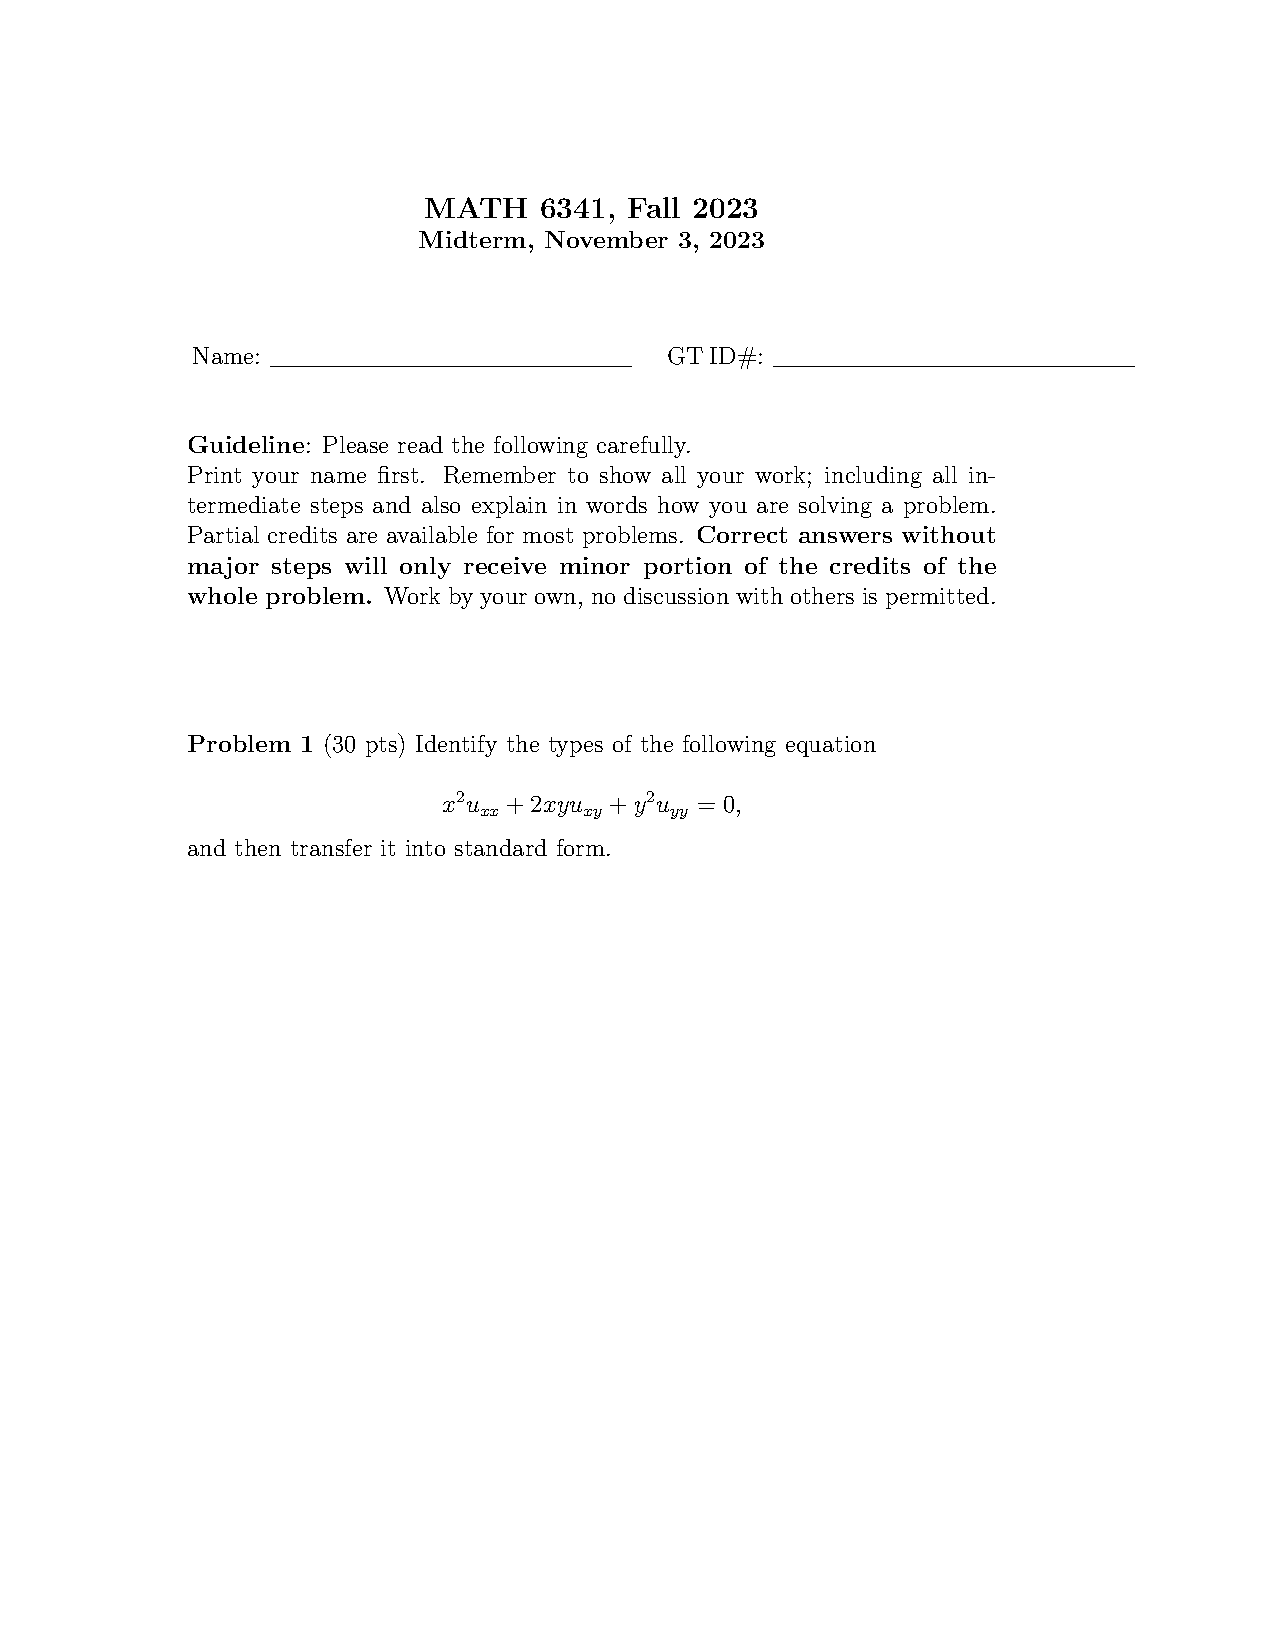
\includepdf[page=-]{Midterm.pdf}
\end{document}
